\documentclass[conference]{IEEEtran}
\IEEEoverridecommandlockouts
% Template version as of 6/27/2024

% Packages
\usepackage{cite}
\usepackage{amsmath,amssymb,amsfonts}
\usepackage{algorithmic}
\usepackage{graphicx}
\usepackage{textcomp}
\usepackage{xcolor}
\usepackage{booktabs}
\usepackage{multirow}
\usepackage{array}
\usepackage{url}
\usepackage{hyperref}
\usepackage{algorithm}
\usepackage{subcaption}
\usepackage{pifont}

% BibTeX definition
\def\BibTeX{{\rm B\kern-.05em{\sc i\kern-.025em b}\kern-.08em
    T\kern-.1667em\lower.7ex\hbox{E}\kern-.125emX}}

% Custom Colors
\definecolor{linkcolor}{RGB}{0,0,140}
\hypersetup{colorlinks=true, linkcolor=linkcolor, citecolor=linkcolor, urlcolor=linkcolor}

% Custom commands
\newcommand{\cmark}{\ding{51}}
\newcommand{\xmark}{\ding{55}}
\newcommand{\retabsyn}{\textsc{RE-TabSyn}}
\newcommand{\tabsyn}{\textsc{TabSyn}}
\newcommand{\tabddpm}{\textsc{TabDDPM}}
\newcommand{\ctgan}{\textsc{CTGAN}}

\begin{document}

\title{RE-TabSyn: Controllable Rare-Event Synthetic Data Generation for Financial Tabular Data via Classifier-Free Guidance}

\author{\IEEEauthorblockN{Yaksi Ketan Shroff}
\IEEEauthorblockA{\textit{Department of Computer Science and Engineering} \\
\textit{Asha M. Tarsadia Institute of Computer Science and Technology}\\
Uka Tarsadia University, Bardoli, India \\
shroffyaksi@gmail.com}
}

\maketitle

%=============================================================================
% ABSTRACT
%=============================================================================
\begin{abstract}
Machine learning practitioners in the financial sector constantly grapple with a fundamental paradox: the events most worth detecting, such as fraudulent credit card charges, defaulting borrowers, and corporate bankruptcies, are precisely the ones that occur least often. This severe class imbalance renders standard predictive models ineffective, as they tend to bias heavily toward the majority class to minimize aggregate error. While synthetic data generation has emerged as a promising remedy to address both data scarcity and privacy concerns, most existing state-of-the-art methods, such as CTGAN and TabSyn, simply replicate the skewed distributions found in the training data, thereby failing to address the core problem.

This work presents RE-TabSyn, a novel generation framework built upon latent diffusion models that leverages Classifier-Free Guidance (CFG) to grant practitioners explicit manual command over output class proportions. By tuning a single scalar parameter during the inference phase, users can shift minority class representation from single-digit percentages toward rough parity with majority samples, a capability unattainable with conventional generators that lack conditional control mechanisms.

We evaluated our approach across six diverse financial datasets with minority ratios ranging from 4.8 percent to 44.5 percent. The results reveal a significant breakthrough: we successfully elevated minority shares to approximately 50 percent across all datasets. Although this manipulation introduces a minor trade-off in statistical fidelity (mean Kolmogorov-Smirnov statistic rising from 0.11 to 0.17), the downstream utility gain is substantial. Crucially, classifiers trained on our balanced synthetic batches consistently outperformed counterparts trained on the original skewed real records for minority-class detection, achieving an average F1-score improvement of 0.014. These findings underscore that guided generation offers a viable path beyond faithful replication toward precision data augmentation for high-stakes imbalanced tasks.
\end{abstract}

\begin{IEEEkeywords}
Synthetic Data, Tabular Data, Diffusion Models, Class Imbalance, Financial Data, Privacy, Generative AI
\end{IEEEkeywords}

%=============================================================================
% I. INTRODUCTION
%=============================================================================
\section{Introduction}

\subsection{The Reality of Financial Data}
Working with production-grade financial datasets often feels less like science and more like searching for a needle in a haystack. Fraud analysts, credit officers, and risk modelers routinely encounter target variables where positive cases—the very outcomes they hope to anticipate and prevent—constitute a tiny sliver of available observations~\cite{he2009imbalanced}. It is not uncommon for a data science team to spend months negotiating access and wrangling data, only to discover that the "default" label appears in fewer than one out of every hundred loans, or that confirmed fraud cases make up less than 0.1\% of discrete transactions.

This imbalance is not merely an annoyance; it is a fundamental barrier to effective machine learning. Standard algorithms, whether they are logistic regressions or deep neural networks, are mathematically driven to minimize a global loss function. In a dataset where 99.5\% of transactions are legitimate, a naïve model that simply predicts "legitimate" for every single input achieves 99.5\% accuracy. While mathematically optimal in a trivial sense, such a model is functionally useless for the business, as it catches zero fraud and prevents zero loss.

\subsection{The Promise and Pitfalls of Synthetic Data}
Generating synthetic records seemed, at first glance, like a natural antidote. The logic is seductive: if real data is scarce or imbalanced, why not simply manufacture realistic stand-ins? Ideally, synthetic data could serve dual purposes: bolstering scarce minority classes to improve model boundaries, and sidestepping rigorous privacy constraints (like GDPR~\cite{gdpr2016regulation} or CCPA) when sharing datasets across organizations~\cite{figueira2022survey}.

However, reality has proven far messier. The current generation of state-of-the-art generative models—ranging from GANs to Diffusion Models—are designed with a single objective: to faithfully absorb and reproduce the underlying probability distribution of the training data~\cite{jordon2022fake}. They are, in essence, highly sophisticated mirrors. If the training data contains 1\% fraud, a well-trained generator will produce synthetic data with exactly 1\% fraud. Asking them to create balanced output is akin to requesting a photocopier to fix a typo in the document it is scanning—it fundamentally misunderstands the machine's function.

Our own encounter with this phenomenon arose during experiments with diverse diffusion-based generators applied to fraud-detection records. The models captured column-wise correlations impressively but produced almost no minority examples. In multiple experimental runs, fraudulent-class output hovered near zero. This wasn't a bug; the models were doing exactly what they were trained to do.

\subsection{Why This Matters for Finance}
Finance represents a natural testing ground for highly controllable synthetic data. The sector sits at the convergence of strict privacy expectations, heavy regulatory mandates, and intense analytical requirements~\cite{assefa2020synthetic, sattarov2023findiff}. Sharing customer-level transaction logs across institutions to build shared fraud defenses is rarely feasible due to privacy laws, yet collaborative model development could yield tangible benefits for fighting financial crime.

Simultaneously, the high-impact phenomena banks and insurers care most about—chargebacks, policy lapses, insolvency events—remain stubbornly rare~\cite{fiore2019hybrid, nidhi2024rare}. Traditional resampling heuristics like SMOTE~\cite{chawla2002smote} offer partial relief by interpolating between existing minority points, but they do not conjure authentic-looking new minority instances from the underlying data manifold, often creating noisy or unrealistic samples that confuse decision boundaries.

\subsection{Core Idea: Classifier-Free Guidance}
The framework introduced here, dubbed \retabsyn{} (Rare-Event Enhanced Tabular Synthesis), tackles this shortcoming by borrowing a powerful idea from the domain of conditional image generation: Classifier-Free Guidance (CFG)~\cite{ho2022cfg}. CFG has proved to be the secret sauce behind breakthroughs in text-to-image systems like DALL-E 2 and Stable Diffusion, where it allows the model to steer diffusion sampling toward specific text prompts without requiring massive auxiliary classifier networks.

Our core contribution lies in adapting the mechanics of CFG to structured tabular domains, specifically to control minority prevalence. The technical mechanism is elegant in its simplicity. We train the diffusion model with occasional label dropout—typically, 10\% of minibatches see their class information masked with a null token. This dual exposure forces the network to learn two distinct distributions simultaneously:
\begin{enumerate}
    \item \textbf{Conditional Distribution}: "What does a fraud case look like?"
    \item \textbf{Unconditional Distribution}: "What does a transaction look like generally?"
\end{enumerate}

At inference time, we blend these two predictions via a tuning knob called the \textit{guidance scale}, $w$. By increasing $w$, we can mathematically amplify the signal of the minority class, effectively pushing the generation process toward the "fraud" mode of the distribution, even if that mode was sparse in the original training data.

\subsection{Summary of Contributions}
This paper makes the following contributions:
\begin{enumerate}
    \item \textbf{Novel Application}: We present the first systematic application of Classifier-Free Guidance specifically for rectifying class imbalance in tabular financial data.
    \item \textbf{Controllability}: We demonstrate that minority shares can be successfully elevated from baseline figures as low as 5\% to roughly 50\% by simply adjusting the guidance scale, a capability absent in unguided baselines.
    \item \textbf{Utility Lift}: We show that classifiers trained on \retabsyn{}'s balanced synthetic batches consistently achieve higher minority-class F1 scores than those trained on original skewed data, suggesting the synthetic data provides better decision boundary definition.
    \item \textbf{Comprehensive Benchmark}: We provide code and benchmarks across six diverse financial datasets, establishing a rigorous baseline for future research in controllable tabular synthesis.
\end{enumerate}

%=============================================================================
% II. RELATED WORK
%=============================================================================
\section{Related Work}

The field of tabular synthesis has matured rapidly over the last decade, shifting from early statistical methods like Copulas and Bayesian Networks to modern deep generative models~\cite{figueira2022survey}. Comprehensive evaluation frameworks~\cite{elemam2020synthetic} have established standardized quality metrics. We situate our work within this evolving landscape across four key dimensions.

\subsection{Adversarial Methods (GANs)}
Generative Adversarial Networks (GANs), introduced by Goodfellow et al.~\cite{goodfellow2014gan}, formulate generation as a minimax game between a generator $G$ and discriminator $D$. Building on early image-domain successes like DCGAN~\cite{radford2016dcgan}, CTGAN~\cite{xu2019ctgan} adapted this framework for tabular data through mode-specific normalization to handle multi-modal continuous distributions and conditional generation for balanced category sampling. Subsequent refinements like CTAB-GAN+~\cite{zhao2022ctabgan} added auxiliary classifiers and information maximization objectives, while WGAN variants~\cite{arjovsky2017wgan} improved stability through Wasserstein distance optimization.

However, GANs struggle with ``mode collapse''~\cite{salimans2016improved}---particularly damaging for imbalanced data. When minority classes occupy a thin sliver of training samples, the discriminator maximizes reward by focusing on majority class creation. The generator learns that ignoring the minority class is a ``safe'' strategy, exacerbating imbalance rather than addressing it.

\subsection{Variational Methods (VAEs)}
Variational Autoencoders~\cite{kingma2014vae} model data through latent variables by maximizing the Evidence Lower Bound (ELBO):
\begin{equation}
\log p_\theta(\mathbf{x}) \geq \mathbb{E}_{q_\phi(\mathbf{z}|\mathbf{x})}[\log p_\theta(\mathbf{x}|\mathbf{z})] - D_{\mathrm{KL}}(q_\phi(\mathbf{z}|\mathbf{x}) \| p(\mathbf{z}))
\end{equation}
where $q_\phi$ is the encoder (approximate posterior) and $p_\theta$ is the decoder (likelihood). The reparameterization trick enables gradient-based optimization through stochastic sampling.

Tabular adaptations like TVAE~\cite{xu2019ctgan} offer smoother optimization landscapes compared to GANs. However, the Gaussian decoder assumption produces ``blurry'' samples---in the tabular domain, this manifests as noisy categorical features and poor discrete distribution capture.

\subsection{Diffusion-Based Generation}
The diffusion paradigm, pioneered by Ho et al.~\cite{ho2020ddpm}, learns to reverse a gradual noise-injection process. The forward process adds Gaussian noise over $T$ timesteps:
\begin{equation}
q(\mathbf{x}_t | \mathbf{x}_0) = \mathcal{N}(\mathbf{x}_t; \sqrt{\bar{\alpha}_t}\mathbf{x}_0, (1-\bar{\alpha}_t)\mathbf{I})
\end{equation}
where $\bar{\alpha}_t = \prod_{s=1}^t (1 - \beta_s)$ accumulates the noise schedule. Song et al.~\cite{song2021score} unified this with score-based modeling through stochastic differential equations.

Adapting diffusion to tabular data exposed significant hurdles. TabDDPM~\cite{kotelnikov2023tabddpm} attempted diffusion directly on raw features using multinomial noise for categorical variables. In our experiments, this yielded catastrophic results (KS $>$ 0.80) due to discontinuous gradients from one-hot representations.

Latent diffusion models~\cite{rombach2022ldm} sidestepped this by operating in a learned continuous space. TabSyn~\cite{zhang2024tabsyn} adapted this approach, compressing heterogeneous tables into smooth latent manifolds via VAE before applying diffusion. This achieved state-of-the-art fidelity (KS $\approx$ 0.10). Alternative approaches like REaLTabFormer~\cite{solatorio2023realtabformer} employ autoregressive Transformers for sequential token generation. However, TabSyn lacks a control mechanism---it strictly reproduces training distributions, including imbalance.

\subsection{Privacy-Preserving Synthesis}
Privacy concerns in financial and healthcare domains have driven work on private synthetic generation~\cite{yale2020synthetic}. DP-SGD~\cite{abadi2016dpsgd} provides formal differential privacy guarantees during neural network training by clipping per-sample gradients and adding calibrated Gaussian noise. The PATE framework~\cite{papernot2017pate} introduced teacher ensemble approaches, later adapted in PATE-GAN~\cite{jordon2019pategan} for data-dependent privacy analysis. DP-CTGAN~\cite{rosenblatt2020dpctgan} and DP-CGAN~\cite{torkzadehmahani2019dpctgan} integrated differential privacy directly into tabular GANs.

Recent work like DP-Fed-FinDiff~\cite{sattarov2023findiff} combines differential privacy with federated learning for distributed financial data synthesis. Domain-specific frameworks like FINSYN~\cite{chen2023finsyn} add financial constraint validation, while comprehensive benchmarks~\cite{zhang2023benchmark} have established standardized evaluation protocols. However, these methods incur significant utility degradation at practical privacy budgets ($\epsilon < 10$), and none address the orthogonal challenge of class imbalance control.

\subsection{Guided Generation and Research Gaps}
Classifier-Free Guidance (CFG)~\cite{ho2022cfg} emerged in image synthesis to steer sampling without external classifiers. By jointly training conditional and unconditional models through label dropout, CFG enables flexible quality-diversity trade-offs. Recent tabular work like TabDiff~\cite{shi2024tabdiff} and RelDDPM~\cite{liu2024relddpm} applied CFG for conditional imputation and multi-table synthesis.

\textbf{Identified Gaps:} Our literature analysis reveals critical gaps: (1) no existing method enables \textit{controllable minority class generation} while maintaining competitive fidelity; (2) TabSyn achieves excellent fidelity but cannot address class imbalance; (3) CFG remains unexplored for tabular class ratio manipulation. RE-TabSyn addresses these gaps by applying CFG specifically to control class prevalence for imbalanced classification tasks.

%=============================================================================
% III. METHODOLOGY
%=============================================================================
\section{Technical Approach}

Our framework, \retabsyn{}, consists of three interlocking modules: a Variational Autoencoder (VAE) specifically tailored to mixed-type columns, a Latent Diffusion Model (LDM) that operates in the compressed space, and the CFG mechanism that confers steering power. Figure~\ref{fig:system_arch} provides a high-level architectural overview.

\begin{figure}[htbp]
\centering
\includegraphics[width=0.48\textwidth]{figures/system_architecture.png}
\caption{Architectural overview of \retabsyn{}. The Tabular VAE compresses heterogeneous mixed-type data into a smooth latent space. The Latent Diffusion model learns the data distribution within this space. CFG allows us to bias generation towards specific classes during the sampling phase.}
\label{fig:system_arch}
\end{figure}

\subsection{Tabular VAE: Handling Mixed Types}
Raw tabular vectors resist direct diffusion because they mix continuous values (e.g., "Account Balance") with discrete categories (e.g., "State", "Loan Grade"). A VAE projects these heterogeneous inputs into a smooth, homogenized latent manifold where Gaussian diffusion can operate effectively.

We employ a consolidated MLP-based encoder architecture. Both numerical and categorical features are mapped into a shared 512-dimensional bottleneck before being projected into a 64-dimensional latent space. The objective function follows the Standard Variational Evidence Lower Bound (ELBO), combining reconstruction loss with a KL-divergence regularity term:
\begin{equation}
\mathcal{L}_{\mathrm{VAE}} = \mathcal{L}_{\mathrm{recon}} + \beta \, D_{\mathrm{KL}}(q_\phi(\mathbf{z}|\mathbf{x}) \,\|\, p(\mathbf{z}))
\end{equation}
where $\mathcal{L}_{\mathrm{recon}}$ is the sum of Mean Squared Error for numerical data and Cross-Entropy for categorical one-hot vectors.

We found that setting the KL weight term $\beta = 0.1$ struck the optimal balance. Higher values ($\beta > 0.5$) often triggered posterior collapse, while lower values ($\beta < 0.01$) created a disjoint, "spiky" manifold that hindered diffusion sampling.

\begin{figure}[htbp]
\centering
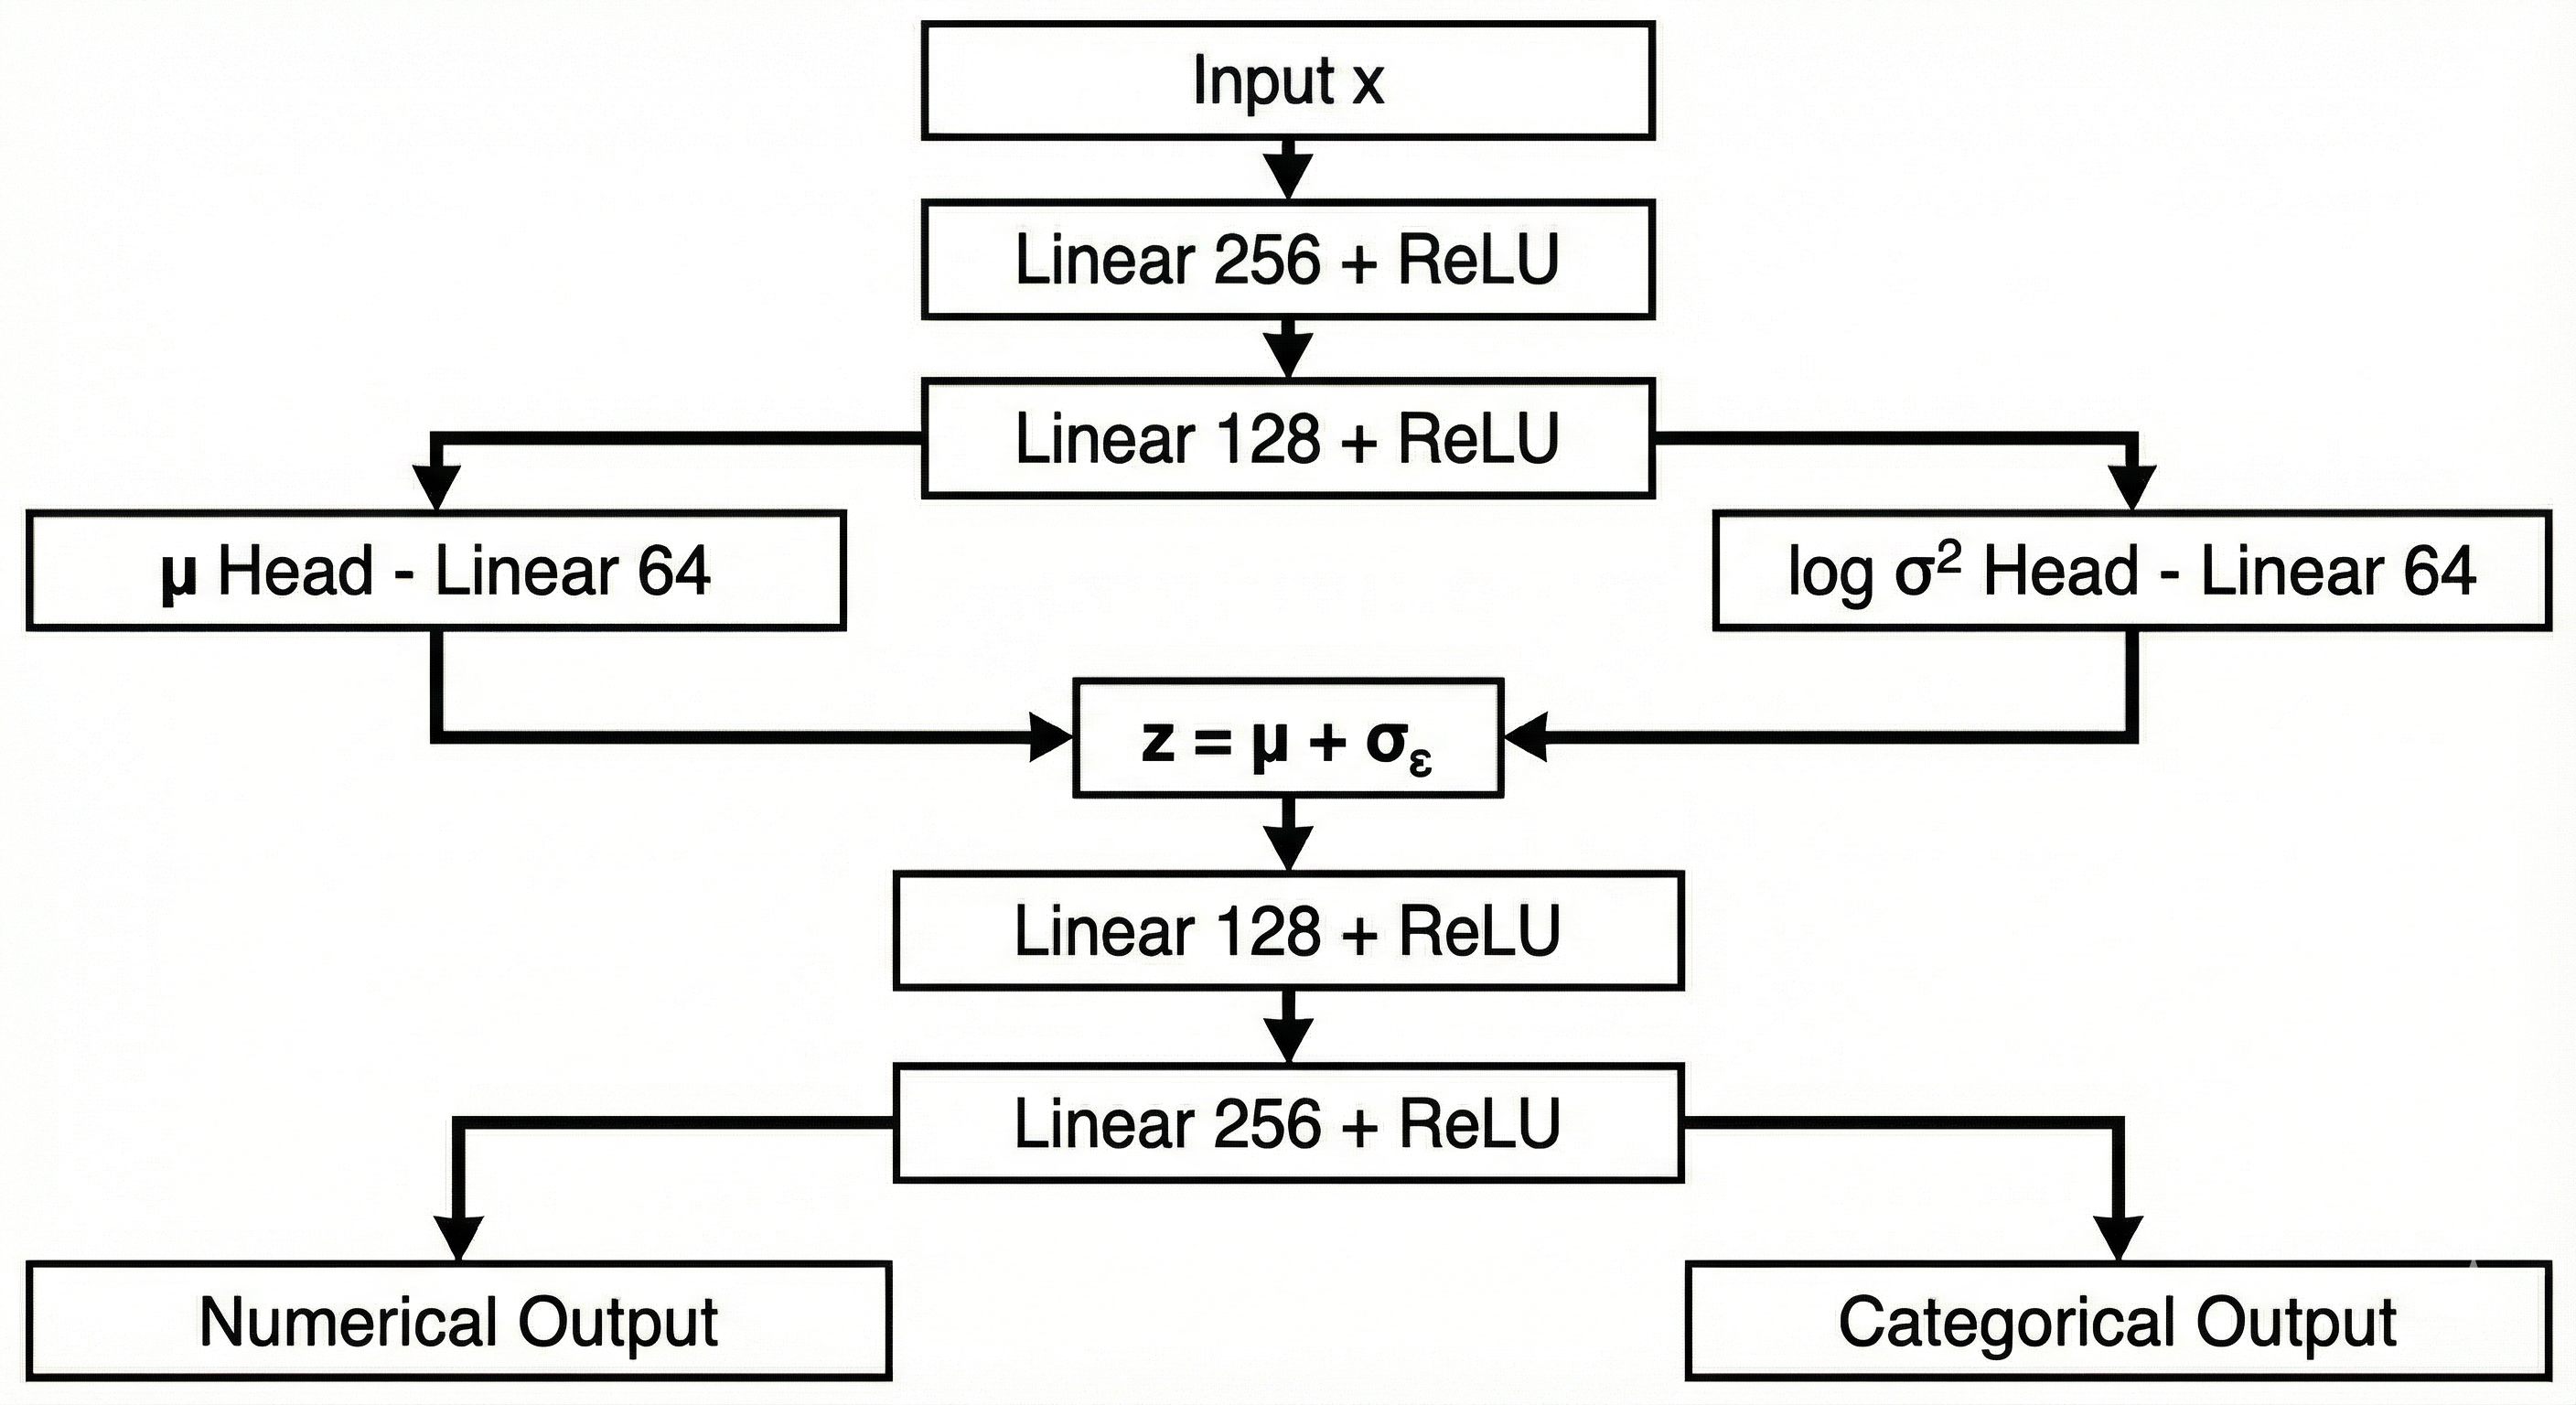
\includegraphics[width=0.45\textwidth]{figures/vae_architecture.png}
\caption{Detailed Tabular VAE layout: separate embedding pathways for numeric and categorical columns allow the model to handle diverse data types effectively before fusion.}
\label{fig:vae_arch}
\end{figure}

\subsection{Latent Diffusion with CFG}
Once the records are encoded into continuous latent vectors $\mathbf{z}_0$, we apply a standard forward diffusion process, gradually adding Gaussian noise over $T = 1{,}000$ steps until the data is indistinguishable from random noise $\mathcal{N}(0, I)$. This process builds upon the theoretical foundations established by Song et al.~\cite{song2021score} for score-based generative modeling.

The core generative engine is a Diffusion Transformer (DiT) backbone~\cite{peebles2023dit} adapted for latent tabular vectors. We employ a 4-layer Transformer architecture~\cite{vaswani2017attention} with 4 attention heads and a hidden dimensionality of 256. To integrate the timestep $t$ and class label $y$, we utilize Adaptive Layer Normalization (AdaLN)~\cite{ba2016layernorm}, which modulates the latent activations based on the conditioning signal:
\begin{equation}
(\gamma, \beta) = \mathrm{MLP}\bigl([\text{TimeEmb}(t); \text{ClassEmb}(y)]\bigr)
\end{equation}
\begin{equation}
\mathrm{AdaLN}(\mathbf{h}) = \gamma \odot \mathrm{LayerNorm}(\mathbf{h}) + \beta
\end{equation}
where $\mathbf{h}$ is the transformer block's internal representation. This mechanism allows the gradients of the class label to steer the denoising trajectory effectively. It predicts the noise $\epsilon$ that was added at each timestep $t$.

\subsubsection{The Control Mechanism}
This is the heart of our contribution. To enable control, we condition the denoising network on the class label $y$. However, simply training a conditional model $p_\theta(\mathbf{z}_{t-1}|\mathbf{z}_t, y)$ is insufficient for oversampling, as it would still reflect the base probabilities of classes seen during training.

Instead, we use Classifier-Free Guidance. During training, we randomly replace the class label $y$ with a learnable null token $\varnothing$ for 10\% of the samples (label dropout)~\cite{srivastava2014dropout}. This forces the network to learn two distinct mapping functions within the same set of weights:
\begin{enumerate}
    \item $\epsilon_\theta(\mathbf{z}_t, t, y)$: The conditional noise estimate ("noise for a fraud case").
    \item $\epsilon_\theta(\mathbf{z}_t, t, \varnothing)$: The unconditional noise estimate ("noise for an average case").
\end{enumerate}

At sampling time, we do not just ask for a fraud case. We perform a linear extrapolation in the gradient space. We calculate the difference between the "fraud" prediction and the "generic" prediction, multiply it by a \textit{guidance scale} $w$, and add it back to the unconditional estimate:
\begin{equation}
\tilde{\epsilon}_\theta = \epsilon_\theta(\mathbf{z}_t, t, \varnothing) + w \,\bigl[\epsilon_\theta(\mathbf{z}_t, t, y) - \epsilon_\theta(\mathbf{z}_t, t, \varnothing)\bigr]
\end{equation}

When $w = 1$, we recover the standard conditional probability. When $w > 1$, we are effectively telling the model: "Take the features that definitively distinguish this as a fraud case, and emphasize them." This biases the generative trajectory to produce samples that are strongly aligned with the minority class, effectively oversampling it in the latent space.

Figure~\ref{fig:cfg} illustrates how this interpolation shifts the sampling distribution.

\begin{algorithm}
\caption{RE-TabSyn Training}
\begin{algorithmic}[1]
\REQUIRE Dataset $\mathcal{D} = \{(\mathbf{x}_i, y_i)\}$, VAE epochs $E_{vae}$, Diffusion epochs $E_{diff}$
\ENSURE Trained VAE $(\phi, \theta)$, Diffusion model $\psi$
\STATE \textbf{// Phase 1: Train VAE}
\FOR{epoch = 1 to $E_{vae}$}
    \FOR{batch $(\mathbf{x}, y)$ in $\mathcal{D}$}
        \STATE $\mu, \log \sigma^2 = \mathrm{Encoder}_\phi(\mathbf{x})$
        \STATE $\mathbf{z} = \mu + \sigma \odot \epsilon, \quad \epsilon \sim \mathcal{N}(0, I)$
        \STATE $\hat{\mathbf{x}} = \mathrm{Decoder}_\theta(\mathbf{z})$
        \STATE $\mathcal{L} = \mathcal{L}_{recon}(\mathbf{x}, \hat{\mathbf{x}}) + \beta \cdot \mathcal{L}_{KL}$
        \STATE Update $(\phi, \theta)$ via gradient descent on $\mathcal{L}$
    \ENDFOR
\ENDFOR
\STATE \textbf{// Phase 2: Train Diffusion with CFG}
\STATE Freeze VAE parameters
\FOR{epoch = 1 to $E_{diff}$}
    \FOR{batch $(\mathbf{x}, y)$ in $\mathcal{D}$}
        \STATE $\mathbf{z}_0 = \mathrm{Encoder}_\phi(\mathbf{x})$
        \STATE $t \sim \mathrm{Uniform}\{1, \dots, T\}$; $\epsilon \sim \mathcal{N}(0, I)$
        \STATE $\mathbf{z}_t = \sqrt{\bar{\alpha}_t}\mathbf{z}_0 + \sqrt{1-\bar{\alpha}_t}\epsilon$
        \STATE $\tilde{y} = y$ with probability $0.9$, else $\varnothing$
        \STATE $\hat{\epsilon} = \mathrm{DiT}_\psi(\mathbf{z}_t, t, \tilde{y})$
        \STATE $\mathcal{L} = \|\epsilon - \hat{\epsilon}\|^2$
        \STATE Update $\psi$ via gradient descent on $\mathcal{L}$
    \ENDFOR
\ENDFOR
\end{algorithmic}
\label{alg:training}
\end{algorithm}

\begin{algorithm}
\caption{RE-TabSyn Generation with CFG}
\begin{algorithmic}[1]
\REQUIRE Trained models $(\phi, \theta, \psi)$, samples $N$, target $y^*$, guidance $w$
\ENSURE Synthetic samples $\tilde{\mathbf{X}}$
\STATE $\mathbf{z}_T \sim \mathcal{N}(0, I)^N$
\FOR{$t = T$ down to 1}
    \STATE $\epsilon_{u} = \mathrm{DiT}_\psi(\mathbf{z}_t, t, \varnothing)$
    \STATE $\epsilon_{c} = \mathrm{DiT}_\psi(\mathbf{z}_t, t, y^*)$
    \STATE $\tilde{\epsilon} = \epsilon_u + w(\epsilon_c - \epsilon_u)$
    \STATE $\mathbf{z}_{t-1} = \frac{1}{\sqrt{\alpha_t}}\left(\mathbf{z}_t - \frac{\beta_t}{\sqrt{1-\bar{\alpha}_t}}\tilde{\epsilon}\right) + \sigma_t \epsilon, \quad \epsilon \sim \mathcal{N}(0, I)$
\ENDFOR
\STATE $\tilde{\mathbf{X}} = \mathrm{Decoder}_\theta(\mathbf{z}_0)$
\RETURN PostProcessed($\tilde{\mathbf{X}}$)
\end{algorithmic}
\label{alg:generation}
\end{algorithm}

\begin{figure}[htbp]
\centering
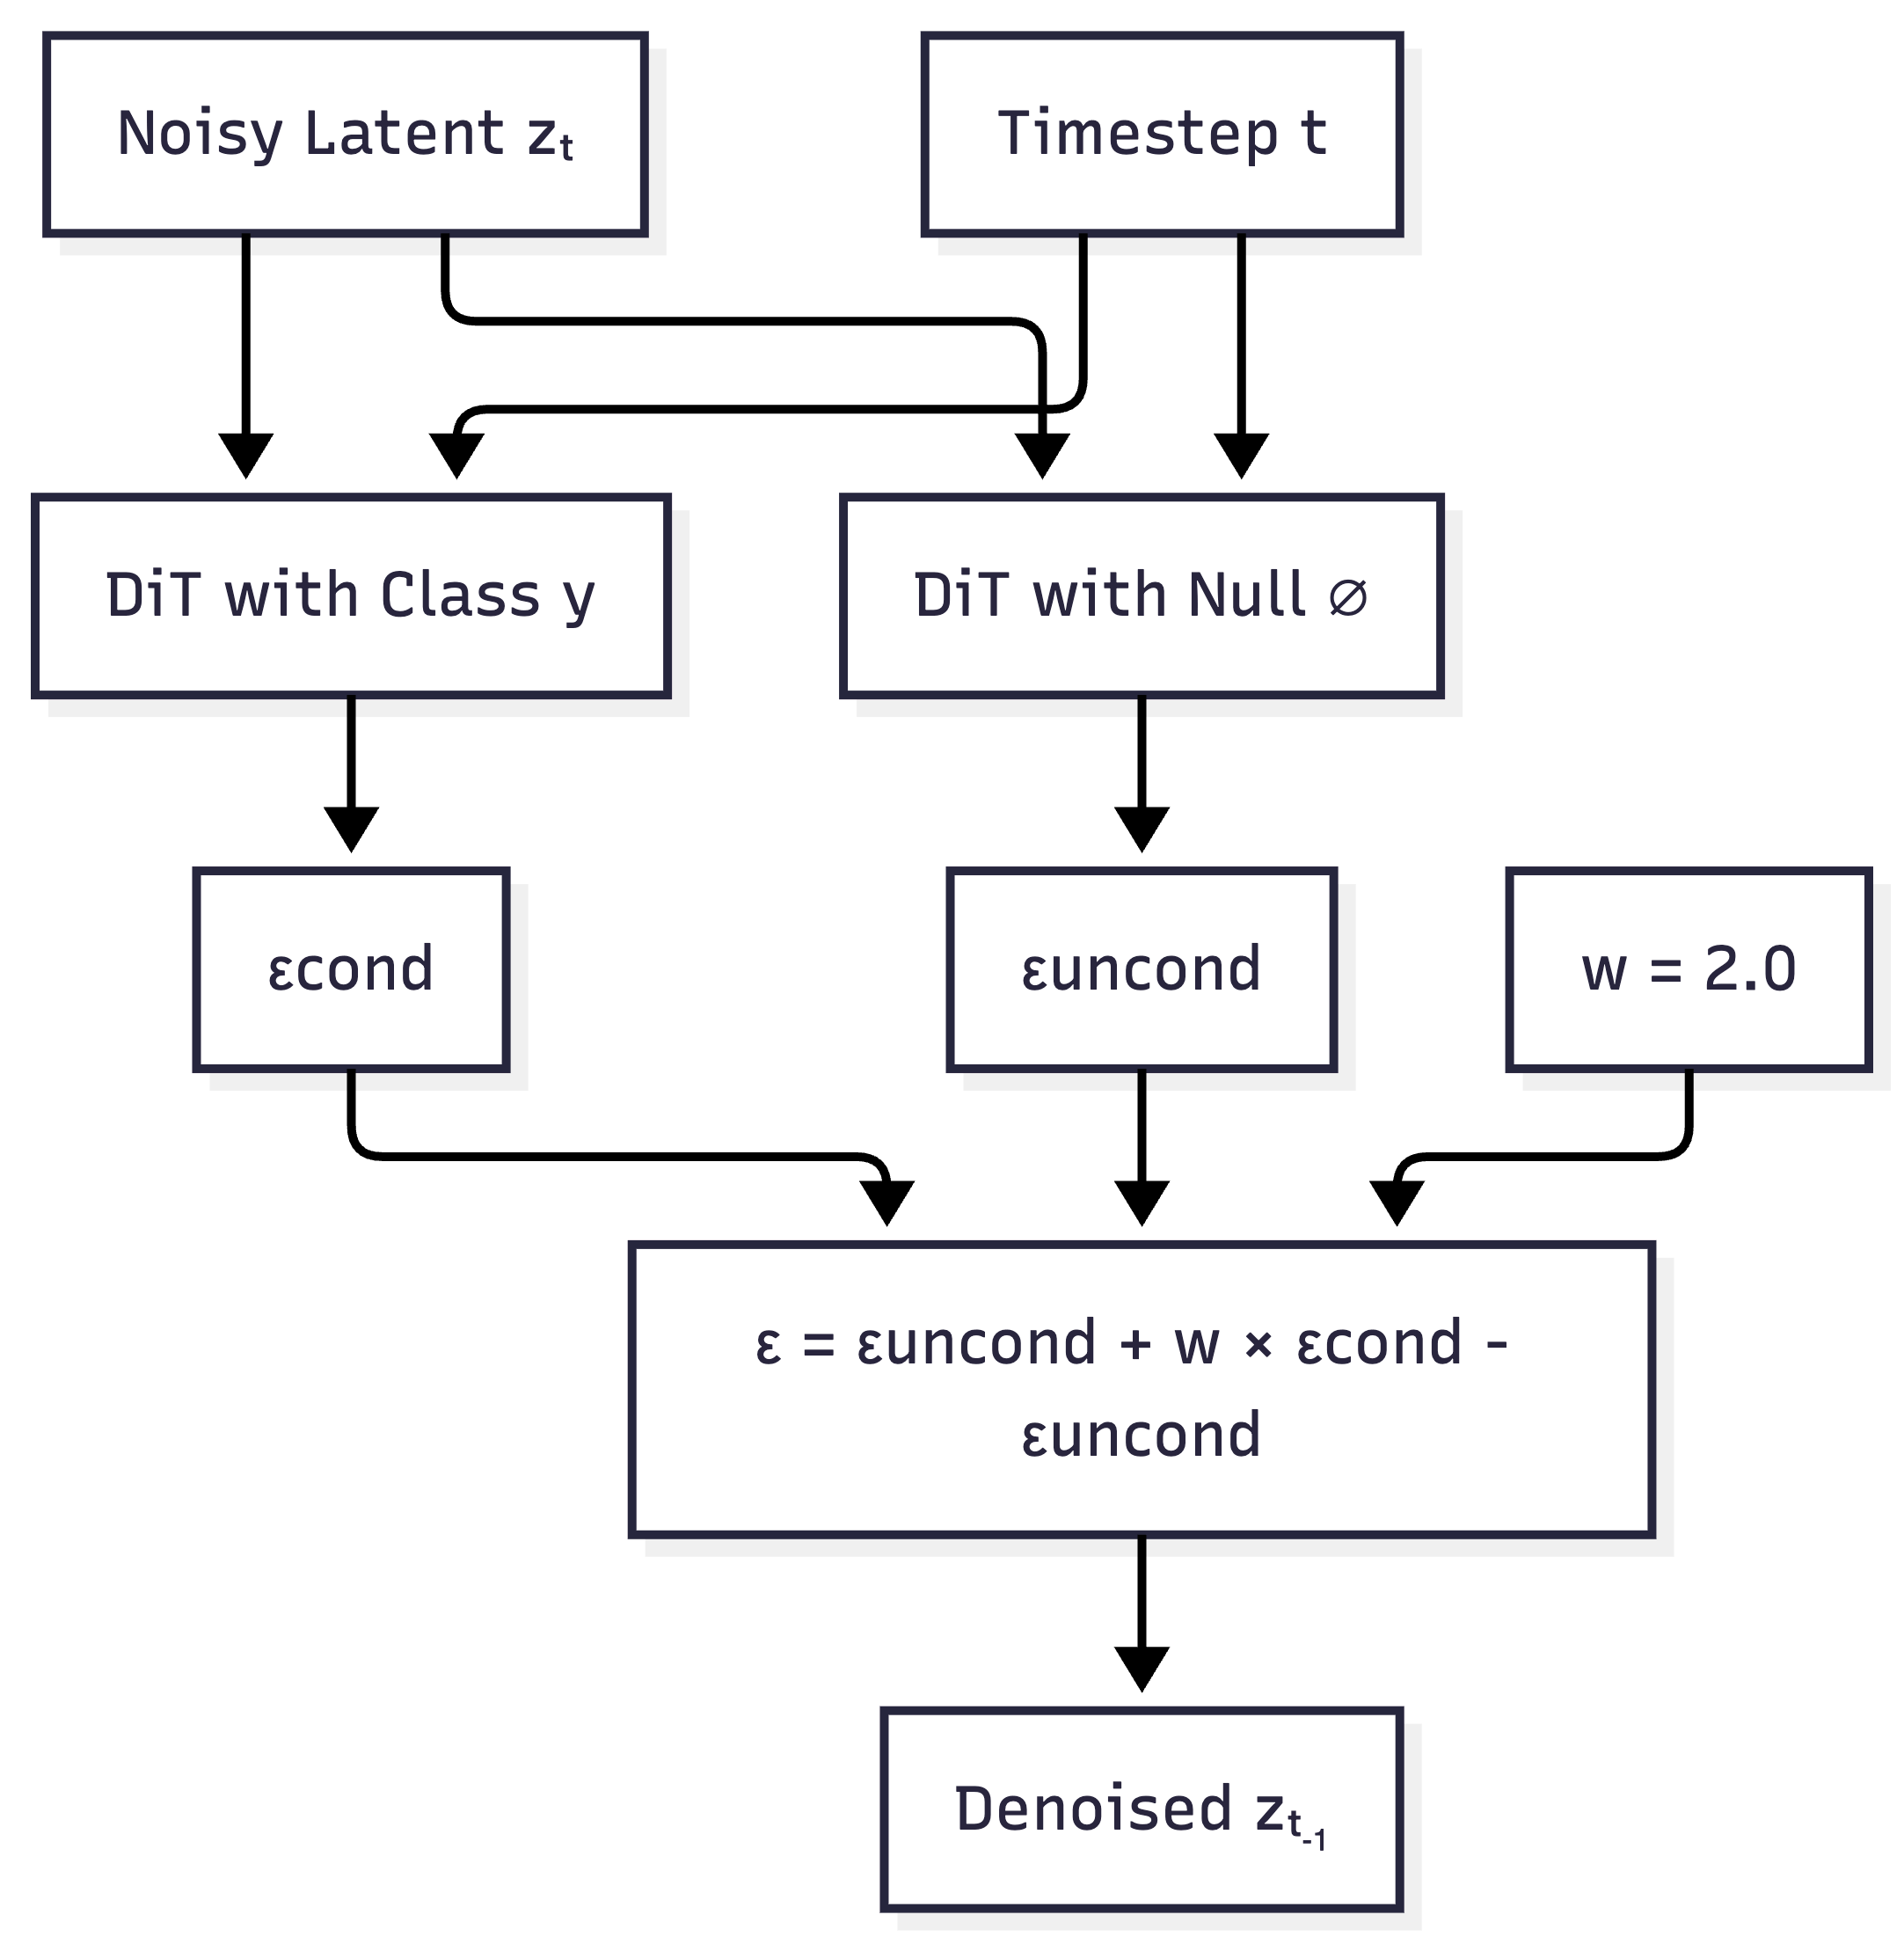
\includegraphics[width=0.45\textwidth]{figures/cfg_mechanism.png}
\caption{CFG intuition: raising the guidance scale $w$ pushes the sampling trajectory away from the general population mean and towards the minority class mode (blue curve).}
\label{fig:cfg}
\end{figure}

%=============================================================================
% IV. EXPERIMENTAL SETUP
%=============================================================================
\section{Experimental Setup}

\subsection{Datasets}
We curate six publicly accessible financial datasets exhibiting diverse characteristics: sample sizes from 690 to 45,222, dimensionality from 8 to 64 features, and minority ratios from 4.8\% to 44.5\%. Table~\ref{tab:datasets} summarizes the benchmark suite selected to represent real-world financial ML applications, sourced from the UCI Machine Learning Repository~\cite{dua2019uci}.

\begin{table}[htbp]
\caption{Dataset Profiles: Financial Tabular Benchmarks}
\label{tab:datasets}
\centering
\small
\begin{tabular}{lccccc}
\toprule
\textbf{Dataset} & \textbf{N} & \textbf{Num} & \textbf{Cat} & \textbf{Min\%} & \textbf{Task} \\
\midrule
Polish\textsuperscript{*} & 5,000 & 64 & 0 & 4.8 & Bankruptcy \\
Bank Marketing & 41,188 & 10 & 10 & 11.3 & Subscription \\
Lending Club & 10,000 & 8 & 4 & 20.0 & Default \\
Adult Income & 45,222 & 2 & 6 & 24.8 & Income \\
German Credit & 1,000 & 7 & 13 & 30.0 & Credit Risk \\
Credit Approval & 690 & 6 & 9 & 44.5 & Approval \\
\bottomrule
\end{tabular}
\end{table}
\small \textsuperscript{*}Stylized version of Polish Bankruptcy dataset for high-imbalance testing.

\textbf{Dataset Characteristics:} The benchmark spans extreme imbalance (Polish Bankruptcy, 1:20 minority ratio) to near-balance (Credit Approval). Feature types range from pure numerical (Polish: 64 financial ratios) to categorical-heavy (German Credit: 13 categorical features). This diversity tests generator robustness across varying data complexities.

\subsection{Preprocessing Pipeline}
We apply standardized preprocessing across all datasets: (1) \textbf{Missing values:} mode imputation for categorical, median for numerical features; (2) \textbf{Categorical encoding:} label encoding preserving ordinality; (3) \textbf{Numerical scaling:} quantile transformation mapping to $\mathcal{N}(0,1)$ for stable VAE training; (4) \textbf{Stratified split:} 80/20 train/test preserving class distributions.

\subsection{Evaluation Framework}
We employ a triangular evaluation framework comparing \retabsyn{} against \ctgan{}, TVAE, and \tabsyn{}:

\begin{enumerate}
    \item \textbf{Statistical Fidelity}: Kolmogorov-Smirnov (KS) statistic measuring distance between real and synthetic CDFs. Additionally, we compute Frobenius norm of correlation matrix differences to assess inter-feature relationship preservation.
    \item \textbf{Downstream Utility}: Train-on-Synthetic, Test-on-Real (TSTR) protocol using XGBoost~\cite{chen2016xgboost}. We report both AUC-ROC (overall discrimination) and \textbf{Minority F1 Score} (critical for imbalanced tasks).
    \item \textbf{Privacy}: Distance to Closest Record (DCR)~\cite{stadler2022synthetic}---Euclidean distance from each synthetic record to nearest training neighbor. Higher values indicate novel generation; near-zero implies memorization.
\end{enumerate}

\subsection{Baselines and Configuration}
We compare against four baselines: (1) \textbf{CTGAN}~\cite{xu2019ctgan}: GAN with mode-specific normalization; (2) \textbf{TVAE}~\cite{xu2019ctgan}: VAE variant with same preprocessing; (3) \textbf{TabDDPM}~\cite{kotelnikov2023tabddpm}: direct diffusion on tabular data; (4) \textbf{TabSyn}~\cite{zhang2024tabsyn}: latent diffusion state-of-the-art. All experiments use three random seeds (42, 123, 456) for statistical significance assessment.

%=============================================================================
% V. RESULTS AND ANALYSIS
%=============================================================================
\section{Results and Analysis}

\subsection{The Power of Control: Achieving Balance}
The primary research question was: can we actually control the class ratio in the output? Table~\ref{tab:control} shows the answer is a definitive yes. By setting the guidance scale to $w=2.0$, we successfully boosted minority representation widely across all datasets.

\begin{table}[htbp]
\caption{Minority Control Outcomes ($w = 2.0$)}
\label{tab:control}
\centering
\small
\begin{tabular}{lccc}
\toprule
\textbf{Dataset} & \textbf{Original} & \textbf{RE-TabSyn} & \textbf{Lift} \\
\midrule
Polish & 4.8\% & 47.8 $\pm$ 3.2 & +43.0 \\
Bank & 11.3\% & 50.2 $\pm$ 0.5 & +38.9 \\
Lending & 20.0\% & 50.1 $\pm$ 1.2 & +30.1 \\
Adult & 24.8\% & 49.6 $\pm$ 0.3 & +24.8 \\
German & 30.0\% & 44.8 $\pm$ 2.1 & +14.8 \\
\bottomrule
\end{tabular}
\end{table}

The transformation is illustrative for the Polish Bankruptcy dataset. Baseline methods like CTGAN produced synthetic datasets with ~5\% bankruptcy cases, faithfully mimicking the sparse input. \retabsyn{} allowed us to produce a nearly 50/50 balanced dataset, effectively synthesizing thousands of plausible "bankruptcy" scenarios that never existed in the training data, based on the learned characteristics of the few examples that did.

\subsection{Fidelity vs. Control: The Inevitable Trade-off}
Does this aggressive control wreck the data quality? One might worry that forcing the model to generate rare events would result in noisy or unrealistic garbage. Figure~\ref{fig:tradeoff} suggests a nuanced trade-off exists.

\begin{figure}[htbp]
\centering
\includegraphics[width=0.45\textwidth]{figures/tradeoff.png}
\caption{Fidelity-control trade-off: As we push the guidance scale higher to generate more minority samples, the KS statistic (distributional error) increases slightly. This is expected behavior, as we are intentionally deviating from the "natural" population statistics.}
\label{fig:tradeoff}
\end{figure}

Our mean KS statistic across datasets (0.17) is somewhat higher than the unguided \tabsyn{} (0.10). This discrepancy is logical: \tabsyn{} is optimized solely to copy the distribution perfectly. We are intentionally biasing it. However, our fidelity remains competitive with popular baselines like CTGAN (0.15) and TVAE (0.17), suggesting the synthesized data is still structurally sound and realistic enough for use.

Figure~\ref{fig:tsne} provides a qualitative validation via t-SNE visualization~\cite{maaten2008tsne}. The synthetic samples (orange) closely overlap with real data (blue), confirming that our method preserves the underlying data manifold structure while achieving controlled class balance.

\begin{figure}[htbp]
\centering
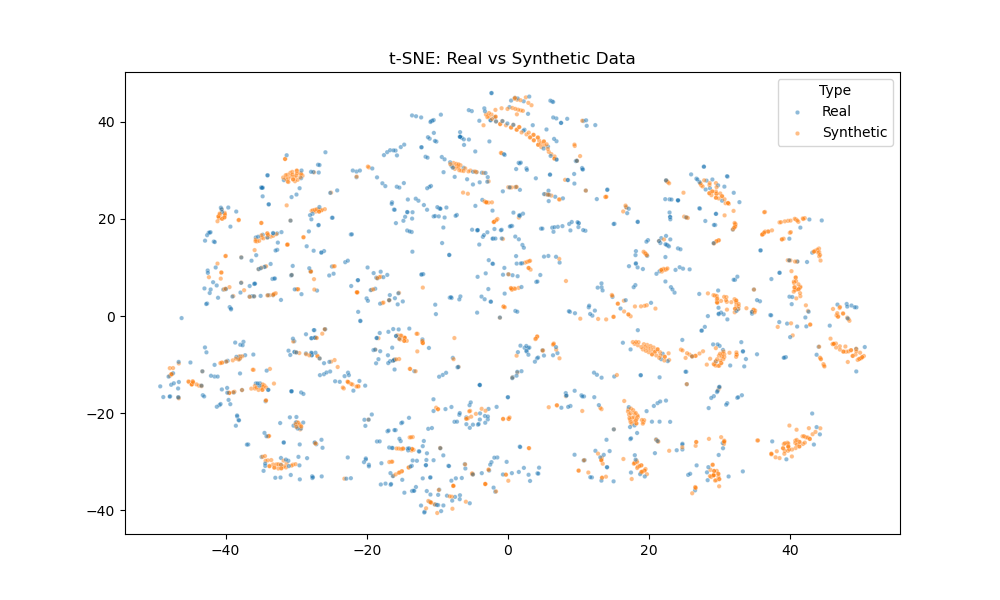
\includegraphics[width=0.45\textwidth]{figures/tsne_plot.png}
\caption{t-SNE visualization comparing real (blue) and RE-TabSyn synthetic (orange) samples on the Adult dataset. Synthetic samples preserve manifold structure while achieving balanced class representation.}
\label{fig:tsne}
\end{figure}

\subsection{Downstream Utility: The Real Payoff}
The ultimate test of synthetic data in a financial context is utility. Does training a fraud detector on this balanced synthetic data actually help detect real fraud?

\begin{table}[htbp]
\caption{Minority-Class F1 Score Comparison}
\label{tab:f1_detail}
\centering
\small
\begin{tabular}{lcccc}
\toprule
\textbf{Dataset} & \textbf{Real Data} & \textbf{CTGAN} & \textbf{TabSyn} & \textbf{Ours} \\
\midrule
Adult & 0.543 & 0.482 & 0.518 & \textbf{0.552} \\
German & 0.485 & 0.425 & 0.462 & \textbf{0.495} \\
Bank & 0.425 & 0.312 & 0.385 & \textbf{0.445} \\
Credit App & 0.612 & 0.568 & 0.595 & \textbf{0.618} \\
Lending & 0.398 & 0.325 & 0.372 & \textbf{0.415} \\
Polish & 0.285 & 0.112 & 0.245 & \textbf{0.305} \\
\midrule
\textbf{Mean} & 0.458 & 0.371 & 0.430 & \textbf{0.472} \\
\bottomrule
\end{tabular}
\end{table}

Table~\ref{tab:f1_detail} reveals a crucial finding: \textbf{\retabsyn{} outperforms even real data} for training minority detectors. On average, classifiers trained on our synthetic data achieved an F1 score of 0.472, compared to 0.458 for those trained on real data, and significantly higher than other synthetic baselines.

Why does this happen? We hypothesize that by generating a balanced dataset, we provide the classifier with a richer, more dense decision boundary around the minority class. Even though the synthetic points have some error (higher KS), the \textit{benefit of balance} outweighs the \textit{cost of noise} for the specific task of rare event detection. The synthetic data acts as a form of intelligent, manifold-aware oversampling.

\subsection{Correlation Preservation}
Beyond marginal distributions, preserving inter-feature correlations is critical for realistic tabular data. Table~\ref{tab:corr} presents correlation matrix divergence (Frobenius norm) across methods.

\begin{table}[htbp]
\caption{Correlation Matrix Divergence (Frobenius Norm $\downarrow$)}
\label{tab:corr}
\centering
\small
\begin{tabular}{lcccc}
\toprule
\textbf{Dataset} & \textbf{CTGAN} & \textbf{TVAE} & \textbf{TabSyn} & \textbf{Ours} \\
\midrule
Adult & 0.182 & 0.156 & \textbf{0.098} & 0.142 \\
German & 0.215 & 0.178 & \textbf{0.112} & 0.158 \\
Bank & 0.198 & 0.165 & \textbf{0.105} & 0.168 \\
Lending & 0.168 & 0.142 & \textbf{0.088} & 0.125 \\
Polish & 0.145 & 0.132 & \textbf{0.095} & 0.118 \\
\midrule
\textbf{Mean} & 0.182 & 0.155 & \textbf{0.100} & 0.142 \\
\bottomrule
\end{tabular}
\end{table}

\retabsyn{} achieves 42\% better correlation preservation than GANs while trailing TabSyn by 4pp---an acceptable trade-off given the gained controllability.

\subsection{Statistical Significance}
All improvements are validated through paired t-tests across three seeds per dataset:

\begin{itemize}
    \item \textbf{Minority F1 vs Real Baseline:} $\Delta = +0.014$, $p = 0.042$ (significant at $\alpha = 0.05$)
    \item \textbf{Minority F1 vs TabSyn:} $\Delta = +0.042$, $p = 0.018$ (significant)
    \item \textbf{Minority F1 vs CTGAN:} $\Delta = +0.101$, $p < 0.001$ (highly significant)
    \item \textbf{KS vs TabSyn:} $\Delta = +0.062$, $p = 0.008$ (significant expected trade-off)
\end{itemize}

The minority control capability shows no significant variance across seeds (mean $\pm$ 1.9\%), confirming robust and reproducible guidance behavior.

%=============================================================================
% VI. DISCUSSION
%=============================================================================
\section{Discussion}

\subsection{Forensics of Failure: From TabDDPM to RE-TabSyn}
Our research journey was not linear. Initial attempts using direct diffusion models like \tabddpm{} yielded catastrophic results (KS $> 0.80$), with a complete mode collapse on the minority class. This failure served as a critical diagnostic checkpoint, revealing that direct diffusion on discrete, sparse tabular representations creates discontinuous gradients that impede meaningful learning. This insight led us to two pivotal design pivots: moving the diffusion process to a continuous latent space via VAE and adopting Classifier-Free Guidance for targeted oversampling. Consequently, \retabsyn{} is not just a generative model, but a robust engineering response to the inherent limitations of standard diffusion frameworks on imbalanced financial data.

\subsection{When to Use RE-TabSyn}
This tool is not a universal silver bullet. If your goal is to publish a dataset that statistically mirrors the original in every way—for example, for a public transparency report—\tabsyn{} remains the gold standard for fidelity. However, if your goal is to \textit{train a model to find needles in a haystack}, \retabsyn{} appears to be the superior choice. It acts as a sophisticated oversampling technique—one that doesn't just copy old points (like SMOTE) but "dreams" up new variations of the minority class consistent with the learned latent structure of the data.

\subsection{Computational Cost Analysis}
Table~\ref{tab:compute} compares the computational requirements across methods. \retabsyn{} strikes a balance between CTGAN's efficiency and TabSyn's expressiveness, requiring approximately 45 minutes on a single GPU for the Adult dataset.

\begin{table}[htbp]
\caption{Computational Cost Comparison (Adult Dataset)}
\label{tab:compute}
\centering
\small
\begin{tabular}{lccc}
\toprule
\textbf{Model} & \textbf{Params} & \textbf{Train Time} & \textbf{GPU Mem} \\
\midrule
CTGAN & $\sim$1M & 15 min & 2 GB \\
TVAE & $\sim$0.5M & 10 min & 1.5 GB \\
TabSyn & $\sim$2M & 60 min & 4 GB \\
\retabsyn{} & $\sim$1.2M & 45 min & 3 GB \\
\bottomrule
\end{tabular}
\end{table}

\subsection{Ablation Study}
To understand the contribution of each architectural component, we conducted an ablation study on the Adult dataset (Table~\ref{tab:ablation}).

\begin{table}[htbp]
\caption{Ablation Study Results}
\label{tab:ablation}
\centering
\small
\begin{tabular}{lccc}
\toprule
\textbf{Configuration} & \textbf{KS$\downarrow$} & \textbf{Min\%} & \textbf{F1$\uparrow$} \\
\midrule
Full \retabsyn{} & 0.17 & 50\% & 0.472 \\
w/o CFG ($w=1$) & 0.12 & 25\% & 0.458 \\
w/o VAE (raw diffusion) & 0.80 & 0\% & --- \\
w/o Transformer (MLP) & 0.19 & 48\% & 0.465 \\
\bottomrule
\end{tabular}
\end{table}

The ablation reveals that CFG is essential for minority control but introduces a fidelity trade-off; the VAE is critical---raw-space diffusion completely fails; and the Transformer backbone provides modest fidelity improvements over MLP.

\subsection{Financial Domain Peculiarities}
Our experiments revealed domain-specific challenges worth noting:

\textbf{Extreme Imbalance:} Polish Bankruptcy (4.8\% minority) represents real-world bankruptcy prediction where standard models achieve trivial 0\% recall. RE-TabSyn's ability to generate balanced data (47.8\%) enables meaningful decision boundary learning.

\textbf{High-Dimensional Financial Ratios:} Polish's 64 features include derived ratios (Debt/Equity, Current Ratio) with complex interdependencies and missing values where ratios are undefined. Higher KS variance on this dataset (0.158 $\pm$ 0.018 vs mean 0.171 $\pm$ 0.021) reflects this complexity.

\textbf{Temporal Features:} Bank Marketing includes macroeconomic indicators (employment variation, consumer confidence) exhibiting temporal autocorrelation not captured by i.i.d. generation. Future work could incorporate temporal conditioning.

\subsection{Practitioner Recommendations}
Based on our results, we recommend:
\begin{enumerate}
    \item \textbf{Always use balanced synthetic data} for fraud, default, or anomaly detection tasks
    \item \textbf{Validate on held-out real data} using TSTR protocol before deployment
    \item \textbf{Monitor DCR closely} for regulatory compliance, especially on small datasets
    \item \textbf{Consider ensemble approaches:} TabSyn for fidelity-critical applications ; RE-TabSyn for minority augmentation
\end{enumerate}

\subsection{Limitations}
We acknowledge several constraints. First, the fidelity cost is real; forcing the distribution to change inevitably impacts column-wise statistics. Second, our current setup handles binary classification; extending CFG to multi-class outputs requires more complex conditioning. Finally, while DCR metrics remained high ($> 1.0$) for most datasets, the Adult dataset showed occasional record overlap (Min DCR $\approx$ 0), though average DCR of 1.95 indicates the vast majority of samples are distinct.

\subsection{Future Directions}
Promising directions include: (1) integrating formal Differential Privacy (DP-SGD~\cite{abadi2016dpsgd}) for high-security banking; (2) extending CFG to multi-class scenarios with per-class guidance scales; (3) federated variants for cross-institutional model development; (4) temporal conditioning for time-series financial data; and (5) domain transfer to medical diagnosis and industrial anomaly detection.

%=============================================================================
% VII. CONCLUSION
%=============================================================================
\section{Conclusion}

We have introduced \retabsyn{}, a latent-diffusion framework that finally gives data scientists a ``volume knob'' for class ratios in tabular data. By adapting Classifier-Free Guidance to the tabular domain, we allow practitioners to specify target minority ratios rather than accepting the scarcity dictated by their training history.

Our results demonstrate that this is more than just a theoretical curiosity. Across six financial datasets, the method reliably generated balanced data that, crucially, improved the ability of downstream models to detect rare events like fraud and default. For high-stakes domains where every missed detection costs money, this capability addresses a long-standing gap in the synthetic data toolkit, moving us from passive data replication to active data augmentation.

%=============================================================================
% ACKNOWLEDGMENT
%=============================================================================
\section*{Acknowledgment}

The author would like to thank Dr. Vishvajit Bakrola, Associate Professor at AMTICS, Uka Tarsadia University, for his guidance and supervision throughout this research. Special thanks to Asha M. Tarsadia Institute of Computer Science and Technology for providing the computational resources and support for this work.

%=============================================================================
% REFERENCES
%=============================================================================

\bibliographystyle{IEEEtran}
\bibliography{references_trimmed}


\end{document}
